\documentclass[lang=cn,11pt,a4paper,cite=authoryear,twocolumn]{elegantpaper}

% 微分号
\newcommand{\dd}[1]{\mathrm{d}#1}
\newcommand{\pp}[1]{\partial{}#1}

\newcommand{\homep}[1]{\Large\textbf{Problem #1}}
\newcommand{\subhome}[1]{\large\textbf{SubProblem #1}}

% FT LT ZT
\newcommand{\ft}[1]{\mathscr{F}[#1]}
\newcommand{\fta}{\xrightarrow{\mathscr{F}}}
\newcommand{\lt}[1]{\mathscr{L}[#1]}
\newcommand{\lta}{\xrightarrow{\mathscr{L}}}
\newcommand{\zt}[1]{\mathscr{Z}[#1]}
\newcommand{\zta}{\xrightarrow{\mathscr{Z}}}

% 积分求和号

\newcommand{\dsum}{\displaystyle\sum}
\newcommand{\aint}{\int_{-\infty}^{+\infty}}

% 简易图片插入
\newcommand{\qfig}[3][nolabel]{
  \begin{figure}[!htb]
      \centering
      \includegraphics[width=0.6\textwidth]{#2}
      \caption{#3}
      \label{#1}
  \end{figure}
}

% 表格
\renewcommand\arraystretch{1.5}


% 日期

\lstset{
  mathescape=false
}

\title{计算机体系架构\quad 第七周作业}
\author{范云潜 18373486}
\institute{微电子学院 184111 班}
\date{\zhtoday}

\begin{document}

\maketitle

作业内容: 	5.1, 5.2, 5.5, 5.8, 5.11,5.14,5.25	 

% \tableofcontents

\homep{5.1}

comb: a, b, c, h, i, 

seq: f, g, j

both: d, e, k

\homep{5.2}

a: 需要写入寄存器的指令全部错误,即 R 指令,因为寄存器的写使能关闭了。

b: ALU 一直工作在受限的,一些需要其他算数逻辑的指令全部出错,不仅包括运算类的指令,还有和寻址相关的指令。如 \lstinline{beq} 需要 ALUop0 = 1 。

c: R 指令失效,因为其 ALUop1 = 1 。

d: Branch 使得之后的与门输出恒为 0 ,分支失效。

e: 需要读内存的指令失效,因为内存选择的一直是 ALU 通路,无法读出正确数据。

d:写内存指令失效,因为写内存使能关闭了。

\homep{5.5}

对于书中 P315 的表格,可能变长的只有 R 指令,可能因为计算单元的变化造成延时增加,那么延时最长为浮点乘法时:400 - 100 + 600 = 900 ps 

\homep{5.8}

\lstinline{jr} 的流程:取指 \(\rightarrow\) 访问寄存器 \(\rightarrow\) 更新 PC 

电路如 \figref{01} 。

% \qfig[01]{h7p3.png}{}

\begin{figure*}
    \centering
    \caption{Jr 电路}
    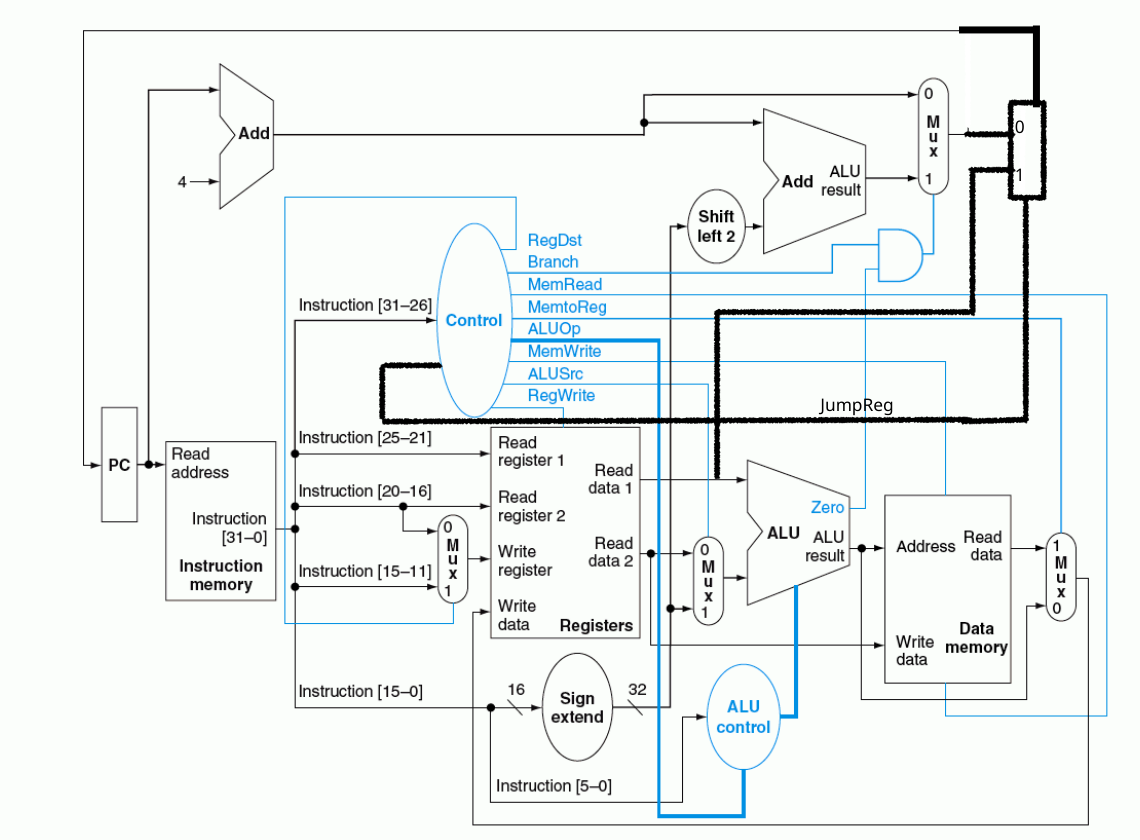
\includegraphics[width=0.9\textwidth]{h7p3.png}
    \label{01}
\end{figure*}

\homep{5.11} 

事实上目前的结构无法在一个周期内对两个寄存器进行读写,因此为了完成这个工作,需要改变寄存器接口,并且为其增加一个 +4 的简单加法器。

首先,增加一个 Write Data2 ,并且扩展 Write Reg 为两位,且在 rt 的 Write Data 添加一个 Mux ,选择 rt 或者 rt + 1 \footnote{疑似书中笔误,我认为 word 地址的相加应该是以 4 为单位的},因此还需要增加一个新的控制信号 Linc 。

\homep{5.14} 

有寄存器:

\begin{lstlisting}
addi $t0, $rs, 0
addi $rs, $rt, 0
addi $rt, $t0, 0
\end{lstlisting}

无寄存器


\begin{lstlisting}
sw $rs, temp 
addi $rs, $rt, 0
lw $rt, temp
\end{lstlisting}

这些实现需要 3 clk ,而硬件需要 1 clk 。3 k + (1 - k) = 1.1 ,那么 k = 0.05 。即只需要 5 \% 的 swap 出现,硬件实现就更好。


\homep{3.25}

\begin{itemize}
    \item Regdst:如果取消,则不能选择写入的寄存器标号。
    \item Branch: 如果取消,无法按照非 +4 的方式改变程序运行方式
    \item MemRead: 可以取消,此时只需让 ReadData恒为对应地址的数据,通过Mem2Reg 和 RegWrite 进行控制
    \item ALUop: 如果取消,无法决定 ALU 的工作状态,改变计算方式
    \item MemWrite: 如果取消,要么无法写入,要么在读取时改变原数据
    \item ALUSrc: 如果取消无法使用立即数
    \item RegWrite: 如果取消无法更改寄存器状态
\end{itemize}


% End Here

\end{document}